\subsection{Final Review}

\content{
        \begin{example}
        Write the number $3042_5$ in base 10.        
        \end{example}
}{% presentation
\vspace{2in}
}{% nopresentation
\vspace{2in}
}{% comments
}

\content{
        \begin{example}
        Write $1024$ in base $6$.
        \end{example}
}{% presentation
\vspace{2in}
}{% nopresentation
\vspace{2in}
}{% comments
}

\content{
        \begin{example}
        Add the following Mayan numerals together. 
        \begin{center}
        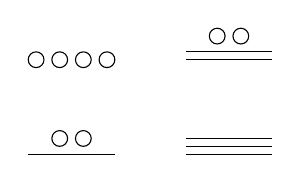
\begin{tikzpicture}
        \draw (-1mm,0) -- (10mm,0);
        \draw (3mm,2mm) circle (1mm);
        \draw (6mm, 2mm) circle (1mm);

        \draw (0mm,12mm) circle (1mm);
        \draw (3mm,12mm) circle (1mm);
        \draw (6mm,12mm) circle (1mm);
        \draw (9mm,12mm) circle (1mm);

        \draw (19mm,0) -- (30mm, 0);
        \draw (19mm,1mm) -- (30mm, 1mm);
        \draw (19mm,2mm) -- (30mm, 2mm);

        \draw (19mm, 12mm) -- (30mm, 12mm);
        \draw (19mm, 13mm) -- (30mm, 13mm);
        \draw (23mm, 15mm) circle (1mm);
        \draw (26mm, 15mm) circle (1mm);
        
        \end{tikzpicture}
        \end{center}
        \end{example}
}{% presentation
}{% nopresentation
}{% comments
}

\content{
        \begin{example}
        Let's remember how shift ciphers work.\\

        \texttt{ABCDEFGHIJKLMNOPQRSTUVWXYZ}\\

        \vspace{-15pt}\hspace{26pt}\texttt{ABCDEFGHIJKLMNOPQRSTUVWXYZ}
        \end{example}
}{% presentation
\vspace{3in}
}{% nopresentation
\vspace{3in}
}{% comments
}

\content{
        \begin{example}
        Encrypt the message ``good luck on the final'' using a
        transposition cipher, and secret key ``lucky''.
        \end{example}
}{% presentation
\vspace{3in}
}{% nopresentation
\vspace{3in}
}{% comments
}

\content{
        \begin{example} The following is an encrypted message using a
        transposition cipher with secret key ``goalie''. What was the message?
        
        \texttt{ntfrin eafsfn leehat tgiaiw}
        \end{example}
}{% presentation
\vspace{3in}
}{% nopresentation
\vspace{3in}
}{% comments
}

\content{
        \begin{example} Your turn! What does the key exchange algorithm look
        like with $p=19$ and $g=13$?
        \end{example}
}{% presentation
\vspace{3in}
}{% nopresentation
\vspace{3in}
}{% comments
}

\content{
        \fbox{\begin{minipage}{\textwidth}
        For these formulas, we have the following: 
        $P_0$ is the principal. 
        $r$ is the interest rate. 
        $t$ is the number of time intervals (specified by problem) which
        have passed. 
        $A$ is the amount paid back.
        $I$ is the interest.

        \begin{center}
        \begin{tabular}{|c|c|}
        \hline
        \T\B Simple Interest &  $ A = P_0(1+r) $ \\
        \hline
        \T\B Simple Interest over Time & $  A = P_0(1+rt) $ \\
        \hline
        \end{tabular}
        \end{center}
        \end{minipage}}
        \fbox{\begin{minipage}{\textwidth}
        For these formulas, we have the following: 
        $P_0$ is the principal, or amount of a loan. 
        $r$ is the annual interest rate.
        $t$ is the number of years which have passed. 
        $A$ is the total amount.
        $k$ is the number of times interest is compounded per year. 
        $d$ is the amount we deposit (or withdraw) from the account regularly,
        or the payment amount on a loan.

        \begin{center}
        \begin{tabular}{|c|c|}
        \hline
        \T\B Compound Interest & $ A =
        P_0\left(1+\frac{r}{k}\right)^{kt} $ \\
        \hline
        \T\B Savings Annuity & $ A =
        d\frac{\left(\left(1+\frac{r}{k}\right)^{kt}-1\right)}{\frac{r}{k}} $\\
        \hline
        \T\B Payout Annuity/Loans & $P_0 =
        d\frac{\left(1-\left(1+\frac{r}{k}\right)^{-kt}\right)}{\frac{r}{k}}$ \\
        \hline
        \end{tabular}
        \end{center}
        \end{minipage}}
}{% presentation
}{% nopresentation
}{% comments
}

\content{
        \begin{example}
        How much do you need in a retirement account to withdraw \$80,000 a year
        for 30 years? Assume that the retirment account earns 5\% interest.
        \end{example}
}{% presentation
\vspace{2in}
}{% nopresentation
\vspace{2in}
}{% comments
}

\content{
        \begin{example}
        Paul wants to save up \$10,000 in 5 years. How much will he need to
        deposit a month in an account earning 4\% to achieve this?
        \end{example}
}{% presentation
\vspace{2in}
}{% nopresentation
\vspace{2in}
}{% comments
}

\content{
        \begin{example}
        If you open an account with 5\% interest, how much will you need to
        deposit when the account opens in order to have \$20,000 in 20 years?
        \end{example}
}{% presentation
\vspace{2in}
}{% nopresentation
\vspace{2in}
}{% comments
}

\content{
        \begin{example}
        Miles is going to take out a loan for a new car, if she can afford \$235
        monthly payments, how big a loan can she take out if the loan earns 3\%
        interest and is 5 years long?
        \end{example}
}{% presentation
\vspace{2in}
}{% nopresentation
\vspace{2in}
}{% comments
}

